\hbadness=10007 \vbadness=10007
\documentclass[journal,12pt,twocolumn]{IEEEtran}
%
\usepackage{circuitikz}
\usepackage{setspace}
\usepackage{textcomp, gensymb}
\usepackage{xcolor}
\usepackage{caption}
%\usepackage{subcaption}
%\doublespacing
\singlespacing

%\usepackage{graphicx}
%\usepackage{amssymb}
%\usepackage{relsize}
\usepackage[cmex10]{amsmath}
\usepackage{mathtools}
%\usepackage{amsthm}
%\interdisplaylinepenalty=2500
%\savesymbol{iint}
%\usepackage{txfonts}
%\restoresymbol{TXF}{iint}
%\usepackage{wasysym}
\usepackage{hyperref}
\usepackage{amsthm}
\usepackage{mathrsfs}
\usepackage{txfonts}
\usepackage{stfloats}
\usepackage{cite}
\usepackage{cases}
\usepackage{subfig}
%\usepackage{xtab}
\usepackage{longtable}
\usepackage{multirow}
%\usepackage{algorithm}
%\usepackage{algpseudocode}
%\usepackage{enumerate}
\usepackage{enumitem}
\usepackage{mathtools}
%\usepackage{iithtlc}
%\usepackage[framemethod=tikz]{mdframed}
\usepackage{listings}
\let\vec\mathbf


%\usepackage{stmaryrd}

%\usepackage{wasysym}
%\newcounter{MYtempeqncnt}
\DeclareMathOperator*{\Res}{Res}
%\renewcommand{\baselinestretch}{2}
\renewcommand\thesection{\arabic{section}}
\renewcommand\thesubsection{\thesection.\arabic{subsection}}
\renewcommand\thesubsubsection{\thesubsection.\arabic{subsubsection}}

\renewcommand\thesectiondis{\arabic{section}}
\renewcommand\thesubsectiondis{\thesectiondis.\arabic{subsection}}
\renewcommand\thesubsubsectiondis{\thesubsectiondis.\arabic{subsubsection}}

%\renewcommand{\labelenumi}{\textbf{\theenumi}}
%\renewcommand{\theenumi}{P.\arabic{enumi}}

% correct bad hyphenation here
\hyphenation{op-tical net-works semi-conduc-tor}

\lstset{
language=Python,
frame=single, 
breaklines=true,
columns=fullflexible
}



\begin{document}
%

\theoremstyle{definition}
\newtheorem{theorem}{Theorem}[section]
\newtheorem{problem}{Problem}
\newtheorem{proposition}{Proposition}[section]
\newtheorem{lemma}{Lemma}[section]
\newtheorem{corollary}[theorem]{Corollary}
\newtheorem{example}{Example}[section]
\newtheorem{definition}{Definition}[section]
%\newtheorem{algorithm}{Algorithm}[section]
%\newtheorem{cor}{Corollary}
\newcommand{\BEQA}{\begin{eqnarray}}
\newcommand{\EEQA}{\end{eqnarray}}
\newcommand{\define}{\stackrel{\triangle}{=}}
\newcommand{\myvec}[1]{\ensuremath{\begin{pmatrix}#1\end{pmatrix}}}
\newcommand{\mydet}[1]{\ensuremath{\begin{vmatrix}#1\end{vmatrix}}}

\bibliographystyle{IEEEtran}
%\bibliographystyle{ieeetr}
\providecommand{\diff}[2]{\ensuremath{\frac{d{#1}}{d{#2}}}}
\providecommand{\nCr}[2]{\,^{#1}C_{#2}} % nCr
\providecommand{\nPr}[2]{\,^{#1}P_{#2}} % nPr
\providecommand{\mbf}{\mathbf}
\providecommand{\pr}[1]{\ensuremath{\Pr\left(#1\right)}}
\providecommand{\qfunc}[1]{\ensuremath{Q\left(#1\right)}}
\providecommand{\sbrak}[1]{\ensuremath{{}\left[#1\right]}}
\providecommand{\lsbrak}[1]{\ensuremath{{}\left[#1\right.}}
\providecommand{\rsbrak}[1]{\ensuremath{{}\left.#1\right]}}
\providecommand{\brak}[1]{\ensuremath{\left(#1\right)}}
\providecommand{\lbrak}[1]{\ensuremath{\left(#1\right.}}
\providecommand{\rbrak}[1]{\ensuremath{\left.#1\right)}}
\providecommand{\cbrak}[1]{\ensuremath{\left\{#1\right\}}}
\providecommand{\lcbrak}[1]{\ensuremath{\left\{#1\right.}}
\providecommand{\rcbrak}[1]{\ensuremath{\left.#1\right\}}}
\theoremstyle{remark}
\newtheorem{rem}{Remark}
\newcommand{\sgn}{\mathop{\mathrm{sgn}}}
\providecommand{\abs}[1]{\left\vert#1\right\vert}
\providecommand{\res}[1]{\Res\displaylimits_{#1}} 
\providecommand{\norm}[1]{\lVert#1\rVert}
\providecommand{\mtx}[1]{\mathbf{#1}}
\providecommand{\mean}[1]{E\left[ #1 \right]}
\providecommand{\fourier}{\overset{\mathcal{F}}{ \rightleftharpoons}}
\providecommand{\ztrans}{\overset{\mathcal{Z}}{ \rightleftharpoons}}

%\providecommand{\hilbert}{\overset{\mathcal{H}}{ \rightleftharpoons}}
\providecommand{\system}{\overset{\mathcal{H}}{ \longleftrightarrow}}
	%\newcommand{\solution}[2]{\textbf{Solution:}{#1}}
\newcommand{\solution}{\noindent \textbf{Solution: }}
\providecommand{\dec}[2]{\ensuremath{\overset{#1}{\underset{#2}{\gtrless}}}}
\numberwithin{equation}{section}
%\numberwithin{equation}{subsection}
%\numberwithin{problem}{subsection}
%\numberwithin{definition}{subsection}
\makeatletter
\@addtoreset{figure}{problem}
\makeatother

\let\StandardTheFigure\thefigure
%\renewcommand{\thefigure}{\theproblem.\arabic{figure}}
\renewcommand{\thefigure}{\theproblem}


%\numberwithin{figure}{subsection}

\def\putbox#1#2#3{\makebox[0in][l]{\makebox[#1][l]{}\raisebox{\baselineskip}[0in][0in]{\raisebox{#2}[0in][0in]{#3}}}}
     \def\rightbox#1{\makebox[0in][r]{#1}}
     \def\centbox#1{\makebox[0in]{#1}}
     \def\topbox#1{\raisebox{-\baselineskip}[0in][0in]{#1}}
     \def\midbox#1{\raisebox{-0.5\baselineskip}[0in][0in]{#1}}

\vspace{3cm}

\title{ 
%\logo{
%}
Circuits and Transforms
%	\logo{Octave for Math Computing }
}
%\title{
%	\logo{Matrix Analysis through Octave}{\begin{center}\includegraphics[scale=.24]{tlc}\end{center}}{}{HAMDSP}
%}


% paper title
% can use linebreaks \\ within to get better formatting as desired
%\title{Matrix Analysis through Octave}
%
%
% author names and IEEE memberships
% note positions of commas and nonbreaking spaces ( ~ ) LaTeX will not break
% a structure at a ~ so this keeps an author's name from being broken across
% two lines.
% use \thanks{} to gain access to the first footnote area
% a separate \thanks must be used for each paragraph as LaTeX2e's \thanks
% was not built to handle multiple paragraphs
%

\author{ G V V Sharma$^{*}$ %<-this  stops a space
\thanks{*The author is with the Department
of Electrical Engineering, Indian Institute of Technology, Hyderabad
502285 India e-mail:  gadepall@iith.ac.in.  All content in the manuscript is 
released under GNU GPL.  Free to use for anything. }% <-this % stops a space
%\thanks{J. Doe and J. Doe are with Anonymous University.}% <-this % stops a space
%\thanks{Manuscript received April 19, 2005; revised January 11, 2007.}}
}
% note the % following the last \IEEEmembership and also \thanks - 
% these prevent an unwanted space from occurring between the last author name
% and the end of the author line. i.e., if you had this:
% 
% \author{....lastname \thanks{...} \thanks{...} }
%                     ^------------^------------^----Do not want these spaces!
%
% a space would be appended to the last name and could cause every name on that
% line to be shifted left slightly. This is one of those "LaTeX things". For
% instance, "\textbf{A} \textbf{B}" will typeset as "A B" not "AB". To get
% "AB" then you have to do: "\textbf{A}\textbf{B}"
% \thanks is no different in this regard, so shield the last } of each \thanks
% that ends a line with a % and do not let a space in before the next \thanks.
% Spaces after \IEEEmembership other than the last one are OK (and needed) as
% you are supposed to have spaces between the names. For what it is worth,
% this is a minor point as most people would not even notice if the said evil
% space somehow managed to creep in.



% The paper headers
%\markboth{Journal of \LaTeX\ Class Files,~Vol.~6, No.~1, January~2007}%
%{Shell \MakeLowercase{\textit{et al.}}: Bare Demo of IEEEtran.cls for Journals}
% The only time the second header will appear is for the odd numbered pages
% after the title page when using the twoside option.
% 
% *** Note that you probably will NOT want to include the author's ***
% *** name in the headers of peer review papers.                   ***
% You can use \ifCLASSOPTIONpeerreview for conditional compilation here if
% you desire.




% If you want to put a publisher's ID mark on the page you can do it like
% this:
%\IEEEpubid{0000--0000/00\$00.00~\copyright~2007 IEEE}
% Remember, if you use this you must call \IEEEpubidadjcol in the second
% column for its text to clear the IEEEpubid mark.



% make the title area
\maketitle

%\newpage

\tableofcontents

%\renewcommand{\thefigure}{\thesection.\theenumi}
%\renewcommand{\thetable}{\thesection.\theenumi}

\renewcommand{\thefigure}{\theenumi}
\renewcommand{\thetable}{\theenumi}

%\renewcommand{\theequation}{\thesection}


\bigskip

\begin{abstract}
This manual provides a simple introduction to Transforms
\end{abstract}


%% Copyright (C) 2020 Saurabh Joshi
%% 
%\let\negmedspace\undefined
%\let\negthickspace\undefined

%\documentclass[journal,12pt,onecolumn]{IEEEtran}
%%\documentclass[journal,12pt,twocolumn]{IEEEtran}
%%
%\usepackage{setspace}
%\usepackage{gensymb}
%%\doublespacing
%\singlespacing
%
%%\usepackage{graphicx}
%%\usepackage{amssymb}
%%\usepackage{relsize}
%\usepackage[cmex10]{amsmath}
%%\usepackage{amsthm}
%%\interdisplaylinepenalty=2500
%%\savesymbol{iint}
%%\usepackage{txfonts}
%%\restoresymbol{TXF}{iint}
%%\usepackage{wasysym}
%\usepackage{amsthm}
%\usepackage{mathrsfs}
%\usepackage{txfonts}
%\usepackage{stfloats}
%\usepackage{cite}
%\usepackage{cases}
%\usepackage{subfig}
%%\usepackage{xtab}
%\usepackage{longtable}
%\usepackage{multirow}
%%\usepackage{algorithm}
%%\usepackage{algpseudocode}
%\usepackage{enumitem}
%\usepackage{mathtools}
% \usepackage{tikz}
%\usetikzlibrary{shapes,arrows,positioning}
% \usepackage{circuitikz}
%\usepackage{verbatim}
%\usepackage{hyperref}
%%\usepackage{stmaryrd}
%\usepackage{tkz-euclide} % loads  TikZ and tkz-base
%%\usetkzobj{all}
%\usepackage{listings}
%    \usepackage{color}                                            %%
%    \usepackage{array}                                            %%
%    \usepackage{longtable}                                        %%
%    \usepackage{calc}                                             %%
%    \usepackage{multirow}                                         %%
%    \usepackage{hhline}                                           %%
%    \usepackage{ifthen}                                           %%
%  %optionally (for landscape tables embedded in another document): %%
%    \usepackage{lscape}     
%\usepackage{multicol}
%\usepackage{chngcntr}
%\usepackage{iftex}
%%\usepackage[latin9]{inputenc}
%\usepackage{geometry}
%%\geometry{verbose,tmargin=2cm,bmargin=3cm,lmargin=1.8cm,rmargin=1.5cm,headheight=2cm,headsep=2cm,footskip=3cm}
%\usepackage{array}
%\newcolumntype{L}[1]{>{\raggedright\let\newline\\\arraybackslash\hspace{0pt}}m{#1}}
%\newcolumntype{C}[1]{>{\centering\let\newline\\\arraybackslash\hspace{0pt}}m{#1}}
%\newcolumntype{R}[1]{>{\raggedleft\let\newline\\\arraybackslash\hspace{0pt}}m{#1}}
% \usepackage{float}
%%\usepackage{graphicx}
%%\usepackage{setspace}
%%\usepackage{parskip}
%
%\def \hsp {\hspace{3mm}}
%
%\makeatletter
%
%\providecommand{\tabularnewline}{\\}
%
%
%\makeatother
%\ifxetex
%\usepackage[T1]{fontenc}
%\usepackage{fontspec}
%%\setmainfont[ Path = fonts/]{Sanskrit_2003.ttf}
%\newfontfamily\nakulafont[Script=Devanagari,AutoFakeBold=2,Path = fonts/]{Nakula}
%%\newfontfamily\liberationfont{Liberation Sans Narrow}
%%\newfontfamily\liberationsansfont{Liberation Sans}
%\fi
% \usepackage{tikz}
%\usepackage{xcolor}
%%\usepackage{enumerate}
%
%%\usepackage{wasysym}
%%\newcounter{MYtempeqncnt}
%\DeclareMathOperator*{\Res}{Res}
%%\renewcommand{\baselinestretch}{2}
%\renewcommand\thesection{\arabic{section}}
%\renewcommand\thesubsection{\thesection.\arabic{subsection}}
%\renewcommand\thesubsubsection{\thesubsection.\arabic{subsubsection}}
%
%\renewcommand\thesectiondis{\arabic{section}}
%\renewcommand\thesubsectiondis{\thesectiondis.\arabic{subsection}}
%\renewcommand\thesubsubsectiondis{\thesubsectiondis.\arabic{subsubsection}}
%
%% correct bad hyphenation here
%\hyphenation{op-tical net-works semi-conduc-tor}
%\def\inputGnumericTable{}                                 %%
%
%\lstset{
%language=tex,
%frame=single, 
%breaklines=true
%}
%
%%\begin{document}
%%
%
%
%\newtheorem{theorem}{Theorem}[section]
%\newtheorem{problem}{Problem}
%\newtheorem{proposition}{Proposition}[section]
%\newtheorem{lemma}{Lemma}[section]
%\newtheorem{corollary}[theorem]{Corollary}
%\newtheorem{example}{Example}[section]
%\newtheorem{definition}[problem]{Definition}
%%\newtheorem{thm}{Theorem}[section] 
%%\newtheorem{defn}[thm]{Definition}
%%\newtheorem{algorithm}{Algorithm}[section]
%%\newtheorem{cor}{Corollary}
%\newcommand{\BEQA}{\begin{eqnarray}}
%\newcommand{\EEQA}{\end{eqnarray}}
%\newcommand{\define}{\stackrel{\triangle}{=}}
%
%\bibliographystyle{IEEEtran}
%%\bibliographystyle{ieeetr}
%
%
%\providecommand{\mbf}{\mathbf}
%\providecommand{\pr}[1]{\ensuremath{\Pr\left(#1\right)}}
%\providecommand{\qfunc}[1]{\ensuremath{Q\left(#1\right)}}
%\providecommand{\sbrak}[1]{\ensuremath{{}\left[#1\right]}}
%\providecommand{\lsbrak}[1]{\ensuremath{{}\left[#1\right.}}
%\providecommand{\rsbrak}[1]{\ensuremath{{}\left.#1\right]}}
%\providecommand{\brak}[1]{\ensuremath{\left(#1\right)}}
%\providecommand{\lbrak}[1]{\ensuremath{\left(#1\right.}}
%\providecommand{\rbrak}[1]{\ensuremath{\left.#1\right)}}
%\providecommand{\cbrak}[1]{\ensuremath{\left\{#1\right\}}}
%\providecommand{\lcbrak}[1]{\ensuremath{\left\{#1\right.}}
%\providecommand{\rcbrak}[1]{\ensuremath{\left.#1\right\}}}
%\theoremstyle{remark}
%\newtheorem{rem}{Remark}
%\newcommand{\sgn}{\mathop{\mathrm{sgn}}}
%\providecommand{\abs}[1]{\left\vert#1\right\vert}
%\providecommand{\res}[1]{\Res\displaylimits_{#1}} 
%\providecommand{\norm}[1]{\left\lVert#1\right\rVert}
%%\providecommand{\norm}[1]{\lVert#1\rVert}
%\providecommand{\mtx}[1]{\mathbf{#1}}
%\providecommand{\mean}[1]{E\left[ #1 \right]}
%\providecommand{\fourier}{\overset{\mathcal{F}}{ \rightleftharpoons}}
%%\providecommand{\hilbert}{\overset{\mathcal{H}}{ \rightleftharpoons}}
%%\providecommand{\system}{\overset{\mathcal{H}}{ \longleftrightarrow}}
%\providecommand{\system}[1]{\overset{\mathcal{#1}}{ \longleftrightarrow}}
%\newcommand{\sinc}{\,\text{sinc}\,}
%\newcommand{\rect}{\,\text{rect}\,}
%	%\newcommand{\solution}[2]{\textbf{Solution:}{#1}}
%\newcommand{\solution}{\noindent \textbf{Solution: }}
%\newcommand{\cosec}{\,\text{cosec}\,}
%\providecommand{\dec}[2]{\ensuremath{\overset{#1}{\underset{#2}{\gtrless}}}}
%\newcommand{\myvec}[1]{\ensuremath{\begin{pmatrix}#1\end{pmatrix}}}
%\newcommand{\mydet}[1]{\ensuremath{\begin{vmatrix}#1\end{vmatrix}}}
%\newcommand*{\permcomb}[4][0mu]{{{}^{#3}\mkern#1#2_{#4}}}
%\newcommand*{\perm}[1][-3mu]{\permcomb[#1]{P}}
%\newcommand*{\comb}[1][-1mu]{\permcomb[#1]{C}}
%%\numberwithin{equation}{section}
%\numberwithin{equation}{section}
%%\numberwithin{problem}{section}
%%\numberwithin{definition}{section}
%\makeatletter
%\@addtoreset{figure}{problem}
%\makeatother
%
%\let\StandardTheFigure\thefigure
%\let\vec\mathbf
%%\renewcommand{\thefigure}{\theproblem.\arabic{figure}}
%\renewcommand{\thefigure}{\theproblem}
%%\setlist[enumerate,1]{before=\renewcommand\theequation{\theenumi.\arabic{equation}}
%%\counterwithin{equation}{enumi}
%
%
%%\renewcommand{\theequation}{\arabic{subsection}.\arabic{equation}}
%
%\vspace{3cm}
%
%
%%\usepackage{babel}
%\begin{document}
%
%\begin{tabular}{L{6cm} C{2cm} R{5cm} }
%
%	\definecolor{circleorange}{rgb}{1,0.17,0.08}
%\definecolor{darkorange}{rgb}{1,0.27,0.1}
%\definecolor{orange2}{rgb}{1,0.5,0.15}
%\definecolor{orange3}{rgb}{1,0.65,0.25}
%\definecolor{yellow1}{rgb}{0.95,0.77,0.2}
%%\begin{tikzpicture}[scale=0.2,every node/.style={transform shape}]
%\begin{tikzpicture}[scale=0.1,every node/.style={transform shape}]
%\draw [fill=circleorange,circleorange] (5,10) circle (1.15); 
%\fill [darkorange] (5.06,8) -- (5.06,2) -- (7.3,1.2) -- (7.3,8.8) -- (5.06,8);
%\fill [darkorange] (4.94,8) -- (4.94,2) -- (2.7,1.2) -- (2.7,8.8) -- (4.94,8);
%\fill [orange2]    (7.4,8.4) -- (7.4,1.6) -- (8.2,1.2) -- (8.2,8.8) -- (7.4,8.4);
%\fill [orange2]    (2.6,8.4) -- (2.6,1.6) -- (1.8,1.2) -- (1.8,8.8) -- (2.6,8.4);
%\fill [orange3]    (8.3,8.4) -- (8.3,1.6) -- (9.0,1.2) -- (9.0,8.8) -- (8.3,8.4);
%\fill [orange3]    (1.7,8.4) -- (1.7,1.6) -- (1.0,1.2) -- (1.0,8.8) -- (1.7,8.4);
%\fill [yellow1]    (9.1,8.4) -- (9.1,1.6) -- (9.7,1.2) -- (9.7,8.8) -- (9.1,8.4);
%\fill [yellow1]    (0.9,8.4) -- (0.9,1.6) -- (0.3,1.2) -- (0.3,8.8) -- (0.9,8.4);
%\ifxetex
%\node [scale=2.1] at (5,-0.1)  {   {\bf {\nakulafont  भारतीय प्रौद्योगिकी संस्थान हैदराबाद }} };
%\node [scale=1.8] at (5,-1.2) {   {\bf { Indian Institute of Technology Hyderabad}} };
%%\node [scale=1.8] at (5,-1.2) {   {\bf {\liberationsansfont Indian Institute of Technology Hyderabad}} };
%\fi
%\end{tikzpicture}
%% \includegraphics[scale=0.05]{logo_iith} \newline
%
%& Quiz  13
%	&
%EE3900	
%\end{tabular}
%
%
%\vspace{-6mm}
%\begin{center}
%%\includegraphics[scale=0.95]{Yellow-Line}
%\begin{tikzpicture}
%\definecolor{yellow1}{rgb}{0.95,0.77,0.2}
%\draw[line width=0.75mm, yellow1] (0,0) -- (\textwidth,0);
%\end{tikzpicture}
%\par\end{center}






%%%%%%%%%%%%%%%%%%%%%%% main %%%%%%%%%%%%%%%%%%%%%%%%%%%%%%%%%%%%%%%%%%
 \section{Definitions}
\begin{enumerate}[label=\arabic*.,ref=\thesection.\theenumi]
\numberwithin{equation}{section}
\numberwithin{figure}{section}
\item The unit step function is 
\begin{align}
u(t) =
\begin{cases}
1 & t > 0
\\
	\frac{1}{2} & t = 0
\\
0 & t < 0
\end{cases}
\end{align}
\item The Laplace transform of $g(t)$ is defined as 
\begin{align}
	G(s) = \int_{-\infty}^{\infty} g(t) e^{-st}\, dt
\end{align}
 \end{enumerate}

 \section{Laplace Transform}
\begin{enumerate}[label=\arabic*.,ref=\thesection.\theenumi]
\numberwithin{equation}{section}
\item In the circuit, the switch S is connected to position P for a long time so that the charge on the capacitor
	becomes $q_1 \, \mu C$. Then S is switched to position Q.  After a long time, the charge on the capacitor is
		$q_2 \, \mu C$.
		\begin{figure}[!ht]
			\centering
			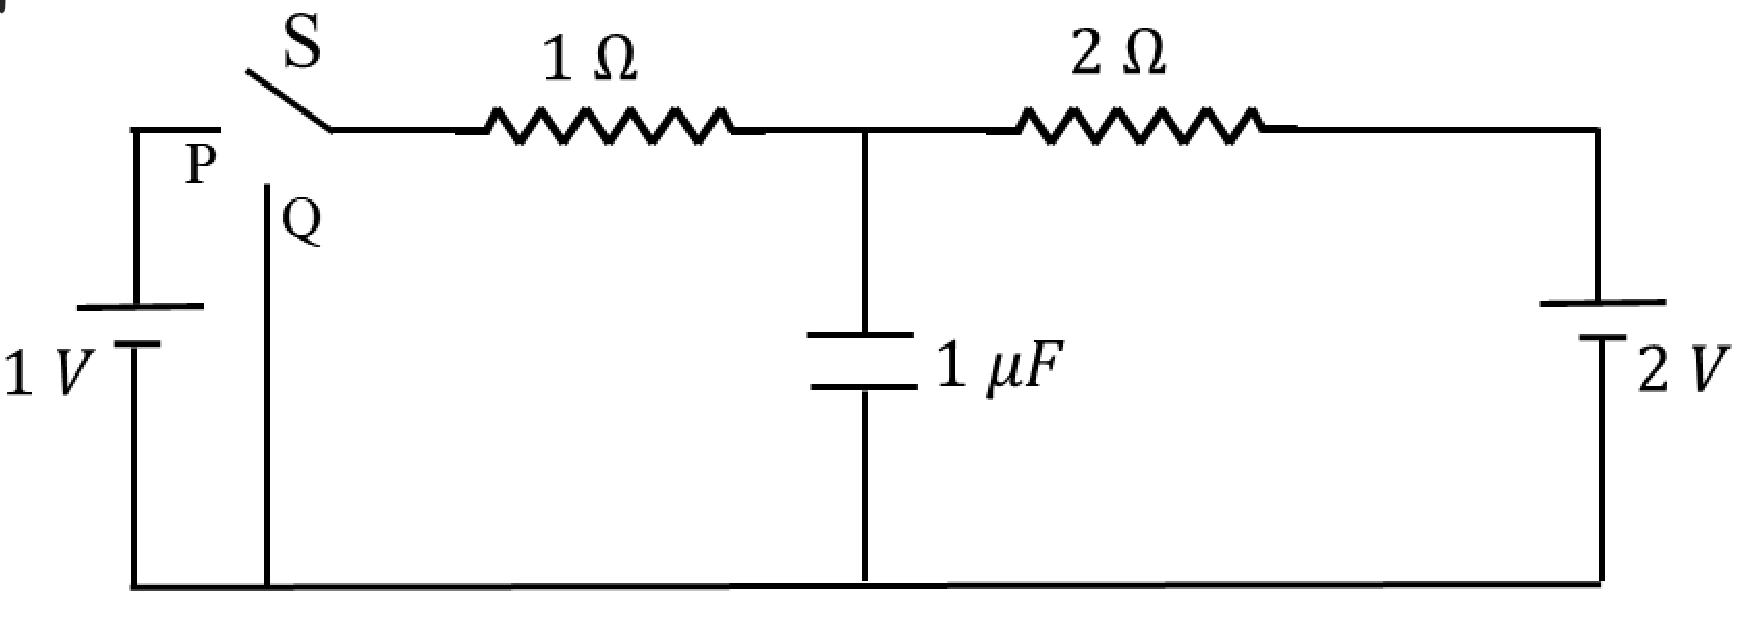
\includegraphics[width=\columnwidth]{figs/ckt.jpg}
			\caption{}
			\label{fig:ckt}
\end{figure}

%%%%%%%%%%%%%%%%%%% 2 %%%%%%%%%%%%%%%%%%%%%%%%%%%%%%%%%%%%%%%%%%%%%%%%%%%%%%%%%%%%%%%

\item Draw the circuit using latex-tikz.\\
\solution\\
The circuit, when the switch S is connected to position P for a long time so that the charge on the capacitor becomes $q_1 \ \mu C$
\begin{figure}[!h]
   \begin{circuitikz}
	   \draw
               (0,0) to[battery1, l=1 $V$, invert] (0,2)
	       -- (0.5,2) node[label={above:P}] {.}
	       -- (1, 2) node[label = {above: S}] {.}
	       to[R, l^=$1 \Omega$] (3,2)
	       to[R, l^=$2 \Omega$] (5.5,2)
	       to[battery1, l=2 $V$] (5.5,0)
	       -- (0,0)
               (3,2) to[C, l=1 ${\mu}F$] (3,0)
	   ;
   \end{circuitikz}
   \caption{}
   \label{fig:ckt-q2}
\end{figure}
%%%%%%%%%%%%%%%%%%%%%%%%%%%%%%%%%%%% question 3 %%%%%%%%%%%%%%%%%%%%%%%%%%%%
\item Find $q_1$.\\
\solution \\
We consider, that the circuit is grounded at G, we use KVL at X to calculate voltage at X, to get voltage over the capacitor.
\begin{figure}[!h]
    \begin{circuitikz} \draw
        (0,0) to[battery1, l=1 $V$, invert] (0,2)
        -- (0.5,2) node[label={above:P}]{}
        to[R, l^=$1 \Omega$] (3,2) 
        node[label={above:X}] {}
        to[R, l^=$2 \Omega$] (5.5,2)
        to[battery1, l=2 $V$] (5.5,0)
        -- (0,0)
        (3,2) to[C, l=1 ${\mu}F$] (3,0) 
        -- (3,-0.5) node[ground, label={right:G}] {};
    \end{circuitikz}
    \caption{}
    \label{fig:ckt-q3}
\end{figure}

\begin{align}
    \frac{V - 1}{1} + \frac{V - 2}{2} = 0 \\
    \implies V = {\frac{4}{3}}\, V
\end{align}
Hence,
\begin{align}
    q_1 = CV = {\frac{4}{3}}{\, \mu C}
\end{align}
%%%%%%%%%%%%%%%%%%%%%%%%%%%%%%%%%%%%%% q4 %%%%%%%%%%%%%%%%%%%%%%%%%%%%%%%%%%%%%%%%%%%
\item Show that the Laplace transform of $u(t)$ is $\frac{1}{s}$ and find the ROC.\\
\solution Applying Laplace transform on $u(t)$,
\begin{align}
	L(u(t)) &= \int_{-\infty}^{\infty}u(t)e^{-st}dt \\
         &= \int_{-\infty}^{0}0.e^{-st}dt + \int_{0}^{\infty}e^{-st}dt \\
         &= \frac{1}{s}, \, \Re{(s)} > 0
         \label{eq:L-u}
\end{align}

%%%%%%%%%%%%%%%%%%%%%%%%%%%%%%%%%%%%% q5 %%%%%%%%%%%%%%%%%%%%%%%%%%%%%%%%%%%%%%%%%%%
\item Show that 
		\begin{align}
			e^{-at}u(t) \stackrel{L}{\longleftrightarrow} \frac{1}{s+a}, \quad a > 0
		\end{align}
and find the ROC.\\
\solution \\
Substitute $s := s + a$ in \eqref{eq:L-u}, and considering
$a \in \mathbb{R}$,

\begin{align}
	e^{-at}u(t) &\stackrel{L}{\longleftrightarrow} \int_{0}^{\infty}u(t)e^{-(s + a)t}dt \\
                &= \frac{1}{s + a}, \quad \Re{(s)} > -a
                \label{eq:L-u-shift}
\end{align}
%%%%%%%%%%%%%%%%%%%%%%%%%%%%%%%%%%%% q6 %%%%%%%%%%%%%%%%%%%%%%%%%%%%%%%%%%%%%%%%%%%
\item Now consider the following resistive circuit transformed from 
			Fig. \ref{fig:ckt}
		\begin{figure}[!ht]
			\centering
			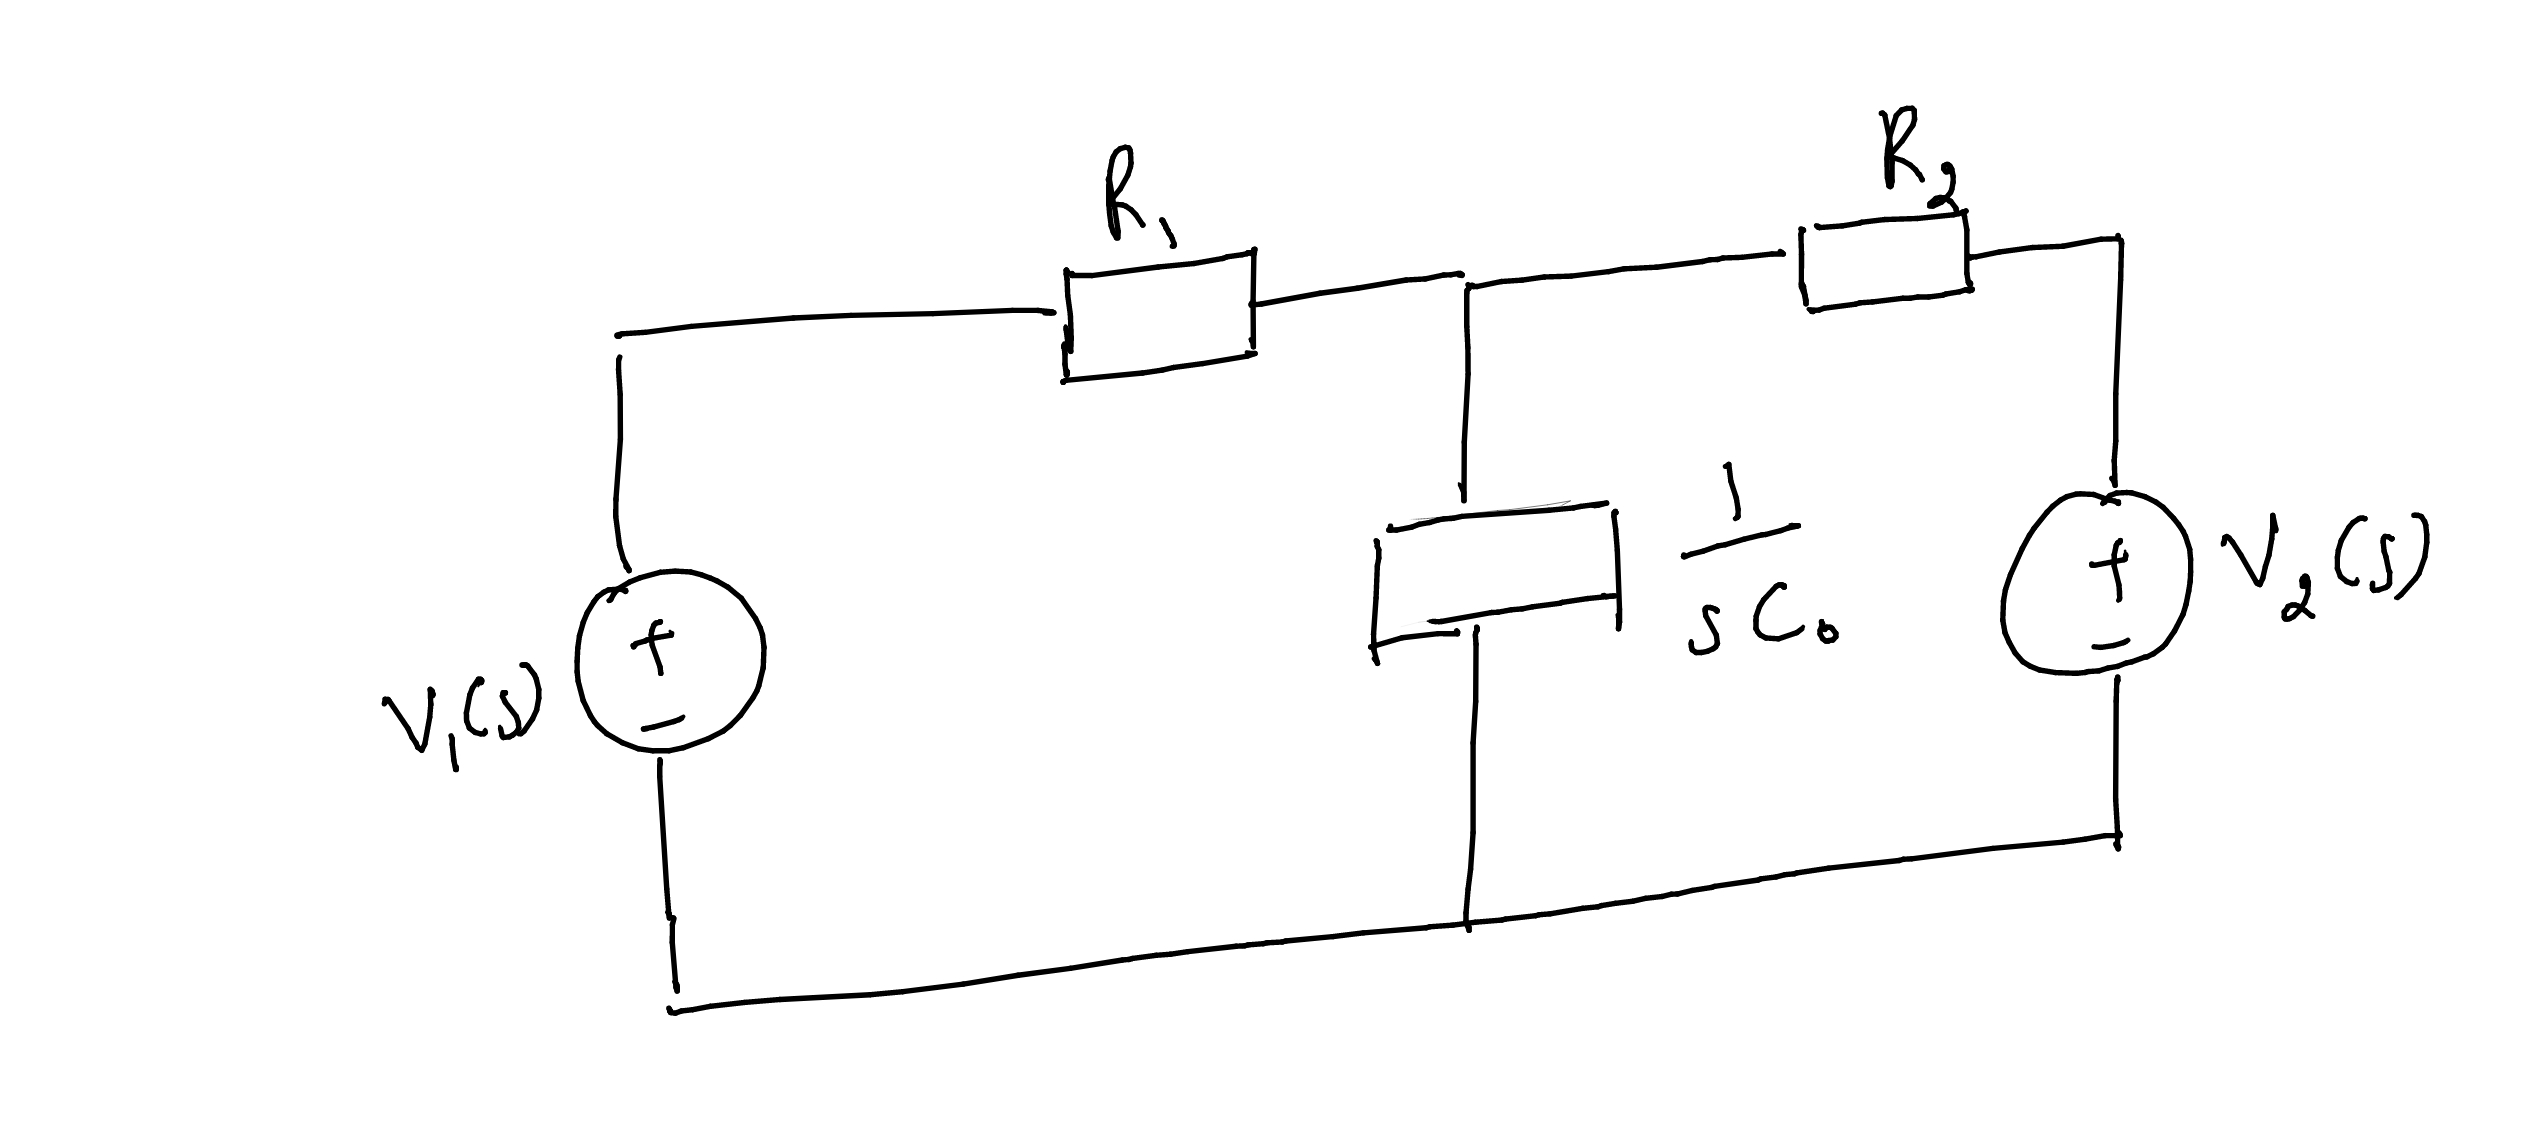
\includegraphics[width=\columnwidth]{figs/lap-ckt.jpg}
			\caption{}
			\label{fig:lap-ckt}
                \end{figure}
where 
		\begin{align}
			u(t) \system{L} V_1(s)
			\\
			2u(t) \system{L} V_2(s)
		\end{align}
Find the voltage across the capacitor $V_{C_0}(s)$.\\
\solution \\
We see that
\begin{align}
    V_1(s) = \frac{1}{s}
    V_2(s) = \frac{2}{s}
\end{align}
Now, labelling points G and X as in Fig. \ref{fig:ckt-q2}, we use KCL at X.

\begin{align}
    &\frac{V - \frac{1}{s}}{R_1} + \frac{V - \frac{2}{s}}{R_2} + sC_0V = 0 \\
    &V\brak{\frac{1}{R_1} + \frac{1}{R_2} + sC_0} = \frac{1}{s}\brak{\frac{1}{R_1} + \frac{2}{R_2}} \\
    &V(s) = \frac{\frac{1}{R_1} + \frac{2}{R_2}}{s\brak{\frac{1}{R_1} + \frac{1}{R_2} + sC_0}} \\
    &= \frac{\frac{1}{R_1} + \frac{2}{R_2}}{\frac{1}{R_1} + \frac{1}{R_2}}\brak{\frac{1}{s} - \frac{1}{\frac{1}{C_0}\brak{\frac{1}{R_1} + \frac{1}{R_2}} + s}} 
    \label{eq:V-cap}
\end{align}



%%%%%%%%%%%%%%%%%%%%%%%%%%%%%%% q7 %%%%%%%%%%%%%%%%%%%%%%%%%%%%%%%%%%%%%%%%%%%%%%%%


\item Find $v_{C_0}(t)$.  Plot using python.\\
\solution \\
Apply inverse Laplace transform to \eqref{eq:V-cap}, \\
we get
\begin{align}
    &V(s) \stackrel{L}{\longleftrightarrow} \frac{2R_1 + R_2}{R_1 + R_2}u(t)\brak{1 - e^{-\brak{\frac{1}{R_1} + \frac{1}{R_2}}\frac{t}{C_0}}} \\
    &= \frac{4}{3}\brak{1 - e^{-\brak{1.5 \times 10^6}t}}u(t)
\end{align}
\begin{figure}[!htb]
    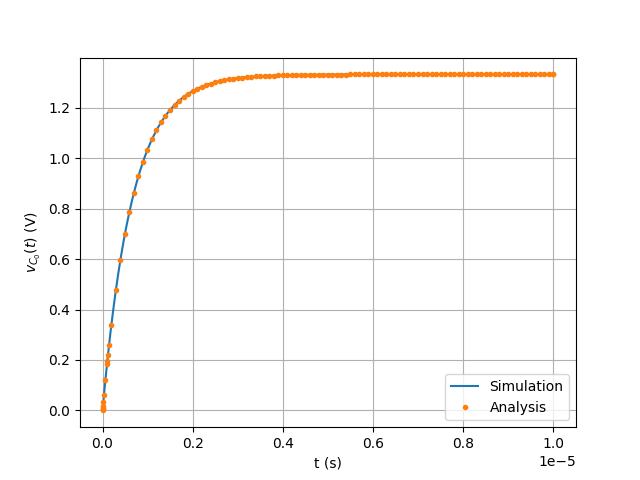
\includegraphics[width=\columnwidth]{figs/2_6.png}
    \caption{$v_{C_0}(t)$ before the switch is flipped}
    \label{fig:v1-t}
\end{figure}
The above graph is plotted using python code codes/2\_7.py
%%%%%%%%%%%%%%%%%%%%%%%%%%%%%%%%% q8 %%%%%%%%%%%%%%%%%%%%%%%%%%%%%%%%%%%%%%%%%%%%%%
\item Verify your result using ngspice.\\
\solution \\ 
The ngspice code in codes/2\_8.cir of the above circuit gives the same output as shown in the plot \eqref{fig:v1-t} above.\\
%%%%%%%%%%%%%%%%%%%%%%%%%%%%%%%% q9 %%%%%%%%%%%%%%%%%%%%%%%%%%%%%%%%%%%%%%%%%%%%%%
	\item Obtain Fig. 
			\ref{fig:lap-ckt}
			using the equivalent differential equation.
\end{enumerate}



%%%%%%%%%%%%%%%%%%%%%%%%%%%%%%%%%%%%% Section 2 %%%%%%%%%%%%%%%%%%%%%%%%%%%%%%%%%%
%%%%%%%%%%%%%%%%%%%%%%%%%%%%%%%%%%%%%%%%%%%%%%%%%%%%%%%%%%%%%%%%%%%%%%%%%%%%%%%%%%%
%%%%%%%%%%%%%%%%%%%%%%%%%%%%%%%%%%%%%%%%%%%%%%%%%%%%%%%%%%%%%%%%%%%%%%%%%%%%%%%%%%


\section{Initial Conditions}
\begin{enumerate}[label=\arabic*.,ref=\thesection.\theenumi]
\numberwithin{equation}{section}
\item Find $q_2$ in Fig. \ref{fig:ckt}.

\solution The equivalent circuit at steady state when the switch is at Q is shown
below.
\begin{figure}[!htb]
    \begin{center}
    \begin{circuitikz} \draw
    (0,0) -- (0,2)
    node[label={above:Q}] {}
    to[R, l^=$1 \Omega$, *-*] (3,2) 
    node[label={above:X}] {}
    to[R, l^=$2 \Omega$] (5.5,2)
    to[battery1, l=2 $V$] (5.5,0)
    -- (0,0)
    (3,2) to[C, l=1 ${\mu}F$] (3,0) 
    -- (3,-0.5) node[ground, label={right:G}] {};
    \end{circuitikz}
    \end{center}
\caption{}
\label{fig:ckt-q2}
\end{figure}

Since capacitor behaves as an open circuit, we use KCL at X.
\begin{align}
    \frac{V - 0}{1} + \frac{V - 2}{2} = 0
    \implies V = {\frac{2}{3}}V
\end{align}                                         
and hence, $q_2 = {\frac{2}{3}}{\mu C}$.

\item Draw the equivalent $s$-domain resistive circuit when S 
is switched to position Q.  Use variables $R_1, R_2, C_0$ for 
the passive elements.	

\begin{figure}[!htb]
    \begin{center}
    \begin{circuitikz} 
    \ctikzset{resistor = european}
    \draw
    (0,0) -- (0,3)
    node[label={above:Q}] {}
    to[R, l^=$R_1$, *-*] (3,3) 
    node[label={above:X}] {}
    to[R, l^=$R_2$] (5.5,3)
    to[battery1, l= $\frac{2}{s} V$] (5.5,0)
    -- (0,0)
    (3,3) to[battery1, l=$\frac{4}{3s} V$] (3,2) to[R, l=$\frac{1}{sC_0}$] (3,0) 
    -- (3,-0.5) node[ground, label={right:G}] {};
    \end{circuitikz}
    \end{center}
\caption{}
\label{fig:sckt-q2}
\end{figure}
\item $V_{C_0}(s)$ = ?  

\solution Using KCL at node X in Fig. \ref{fig:sckt-q2}
\begin{align}
    \frac{V - 0}{R_1} + \frac{V - \frac{2}{s}}{R_2} + sC_0\brak{V - \frac{4}{3s}} = 0 \\
\implies V_{C_0}(s) = \frac{\frac{2}{sR_2} + \frac{4C_0}{3}}{\frac{1}{R_1} + \frac{2}{R_2} + sC_0}
\label{eq:v2-s}
\end{align}
\item $v_{C_0}(t)$ = ? Plot using python.

\solution From \eqref{eq:v2-s},
\begin{align}
    &V_{C_0}(s) = \frac{4}{3}\brak{\frac{1}{\frac{1}{C_0}\brak{\frac{1}{R_1} + \frac{1}{R_2}}+s}} \nonumber \\
    &+ \frac{2}{R_2\brak{\frac{1}{R_1} +\frac{1}{R_2}}}\brak{\frac{1}{s} - \frac{1}{\frac{1}{C_0}\brak{\frac{1}{R_1} + \frac{1}{R_2}} + s}}
\end{align}
Taking an inverse Laplace Transform,
\begin{align}
    &v_{C_0}(t) = \frac{4}{3}e^{-\brak{\frac{1}{R_1} + \frac{1}{R_2}}\frac{t}{C_0}}u(t) \nonumber \\ 
    &+ \frac{2}{R_2\brak{\frac{1}{R_1}+\frac{1}{R_2}}}\brak{1 - e^{-\brak{\frac{1}{R_1} + \frac{1}{R_2}}\frac{t}{C_0}}}u(t)
\end{align}
Substituting values gives
\begin{align}
    v_{C_0}(t) = \frac{2}{3}\brak{1 +e^{-\brak{1.5 \times 10^6}t}}u(t)
    \label{eq:v2-t}
\end{align}
The Python code \texttt{codes/3\_4.py} plots the graph below.
\begin{figure}[!htb]
    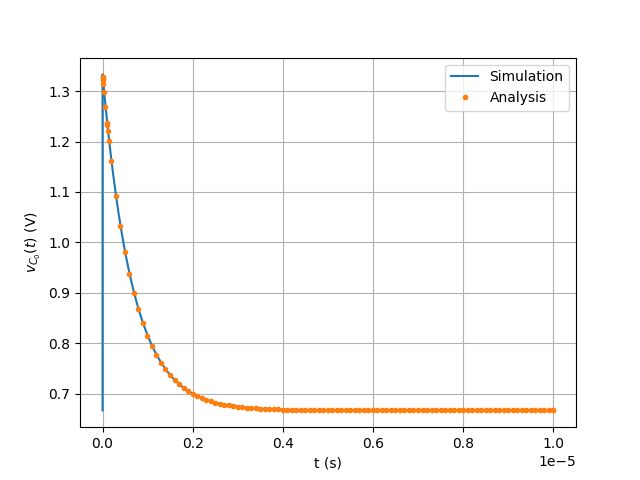
\includegraphics[width=\columnwidth]{figs/3_4.png}
    \caption{$v_{C_0}(t)$ after the switch is flipped}
    \label{fig:v2-t}
\end{figure}
\item Verify your result using ngspice.

\solution The ngspice script \texttt{codes/3\_5.cir} simulates the given circuit and the generated output is depicted in Fig. \eqref{fig:v2-t}.
\item Find $v_{C_0}(0-), v_{C_0}(0+)$ and  $v_{C_0}(\infty) $. 

\solution From the initial conditions,
\begin{align}
    v_{C_0}(0-) = \frac{q_1}{C_0} = {\frac{4}{3}}V
\end{align}

Using \eqref{eq:v2-t},
\begin{align}
    v_{C_0}(0+) &= \lim_{t \to 0+}v_{C_0}(t) = {\frac{4}{3}}V \\
    v_{C_0}(\infty) &= \lim_{t \to \infty}v_{C_0}(t) = {\frac{2}{3}}V
\end{align}

\item Obtain the Fig. in problem 3.2 using the equivalent differential equations.

\solution The equivalent circuit in the $t$-domain is shown below.
	
\begin{figure}[!htb]
    \begin{center}
    \begin{circuitikz} 
    \draw
    (0,0) -- (0,3)
    node[label={above:Q}] {}
    to[R, l^=$R_1$, *-*, i = $i_1$] (3,3) 
    node[label={above:X}] {}
    to[R, l^=$R_2$, i = $i_3$] (5.5,3)
    to[battery1, l= ${2}V$] (5.5,0)
    -- (0,0)
    (3,3) to[battery1, l=$\frac{4}{3} V$] (3,2) to[C, l=$C_0$, i = $i_2$] (3,0) ;
    \end{circuitikz}
    \end{center}
\caption{}
\label{fig:tckt-q2}
\end{figure}
From KCL and KVL,
\begin{align}
    &i_1 = i_2 +i_3 \\
    &i_1R_1 + \frac{4}{3} + \frac{1}{C_0}\int_{0}^{t}i_2dt = 0 \\
    &\frac{4}{3} + \frac{1}{C_0}\int_{0}^{t}i_2dt - i_3R_2 - 2 = 0
\end{align}
Taking Laplace Transforms on both sides and using the properties of Laplace Transforms,
\begin{align}
    &I_1 = I_2 +I_3 \label{eq:s1}\\
    &I_1R_1 + \frac{4}{3} + \frac{1}{sC_0}I_2 = 0 \\
    &\frac{4}{3} + \frac{1}{sC_0}I_2 - I_3R_2 - 2 = 0 \label{eq:s3}
\end{align}
where $i(t) \system{L} I(s)$. Note that the capacitor is equivalent to 
a resistive element of resistance $R_C = \frac{1}{sC_0}$ in the 
$s$-domain. Equations \eqref{eq:s1} - \eqref{eq:s3} precisely describe 
Fig. \ref{fig:sckt-q2}. 
\end{enumerate}

\section{Bilinear Transform}
\begin{enumerate}[label=\arabic*.,ref=\thesection.\theenumi]
\numberwithin{equation}{section}
\item In Fig. \ref{fig:ckt}, consider the case when $S$ is switched to 
$Q$ right in the beginning. Formulate the differential equation.

\solution The equivalent circuit in the $t$-domain is shown below.
	
\begin{figure}[!htb]
    \begin{center}
    \begin{circuitikz} 
    \draw
    (0,0) -- (0,3)
    node[label={above:Q}] {}
    to[R, l^=$R_1$, *-*, i = $i_1$] (3,3) 
    node[label={above:X}] {}
    to[R, l^=$R_2$, i = $i_3$] (5.5,3)
    to[battery1, l= $V_2$] (5.5,0)
    -- (0,0)
    (3,3) to[C, l=$C_0$, i = $i_2$] (3,0) ;
    \end{circuitikz}
    \end{center}
\caption{}
\label{fig:tckt-q4}
\end{figure}

Applying KCL and KVL,
\begin{align}
    &i_1 = i_2 + i_3 \\
    &i_1R_1 + \frac{1}{C_0}\int_0^ti_2\, dt = 0 \\
    &i_3R_2 + 2 - \frac{1}{C_0}\int_0^ti_2\, dt = 0
\end{align}
Differentiating the above equations,
\begin{align}
    &\diff{i_1}{t} = \diff{i_2}{t} + \diff{i_3}{t} \label{eq:diff1}\\
    &R_1\diff{i_1}{t} + \frac{i_2}{C_0} = 0 \label{eq:diff2}\\
    &R_2\diff{i_3}{t} - \frac{i_2}{C_0} = 0 \label{eq:diff3}
\end{align}
Using \eqref{eq:diff1} and \eqref{eq:diff3} in \eqref{eq:diff2},
\begin{align}
    &R_1\brak{\diff{i_2}{t} + \diff{i_3}{t}} + \frac{i_2}{C_0} = 0 \\
    &R_1\diff{i_2}{t} + \brak{1 + \frac{R_1}{R_2}}\frac{i_2}{C_0} = 0 \\
    &\diff{i_2}{t} + \brak{\frac{1}{R_1} + \frac{1}{R_2}}\frac{i_2}{C_0} = 0 \\
    &\diff{i_2}{t} + \frac{i_2}{\tau} = 0
    \label{eq:diff-eqn-init}
\end{align}
where $\tau = \frac{C_0R_1R_2}{R_1 + R_2}$ is the RC time 
constant of the circuit. Note that $i_2(0) = \frac{V_2}{R_2}$ A and 
$i_2 = C_0\diff{V}{t}$, where $V$ is the voltage of the capacitor. 
Hence, integrating \eqref{eq:diff-eqn-init},
\begin{align}
    C_0\diff{V}{t} - \frac{V_2}{R_2} + \frac{C_0V}{\tau} &= 0 \\
    \implies \diff{V}{t} + \frac{V}{\tau} = \frac{V_2}{C_0R_2}
    \label{eq:diff-eqn}
\end{align}
\item Find $H(s)$ considering the output voltage at the capacitor.

\solution Transforming Fig. \ref{fig:tckt-q4} to the $s$-domain,

\begin{figure}[!htb]
    \begin{center}
    \begin{circuitikz} 
    \ctikzset{resistor = european}
    \draw
    (0,0) -- (0,3)
    node[label={above:Q}] {}
    to[R, l^=$R_1$, *-*] (3,3) 
    node[label={above:X}] {}
    to[R, l^=$R_2$] (5.5,3)
    to[battery1, l= $V_2(s)$] (5.5,0)
    -- (0,0)
    (3,3) to[R, l=$\frac{1}{sC_0}$] (3,0) 
    -- (3,-0.5) node[ground, label={right:G}] {};
    \end{circuitikz}
    \end{center}
\caption{}
\label{fig:sckt-q4}
\end{figure}

Applying nodal analysis at X, and noting that 
$H(s) = \frac{V(s)}{V_2(s)}$,
\begin{align}
    &\frac{V}{R_1} + \frac{V}{\frac{1}{sC_0}} + \frac{V - V_2}{R_2} = 0 \\
    &H(s)\brak{\frac{1}{R_1} + \frac{1}{R_2} + sC_0} = \frac{1}{R_2} \\
    &H(s) = \frac{\frac{1}{R_2}}{\frac{1}{R_1} + \frac{1}{R_2} + sC_0}
    \label{eq:Hs}
\end{align}
\item Plot $H(s)$. What kind of filter is it?

\solution The Python code \texttt{codes/4\_3.py} plots $H(s)$.
\begin{figure}[!ht]
    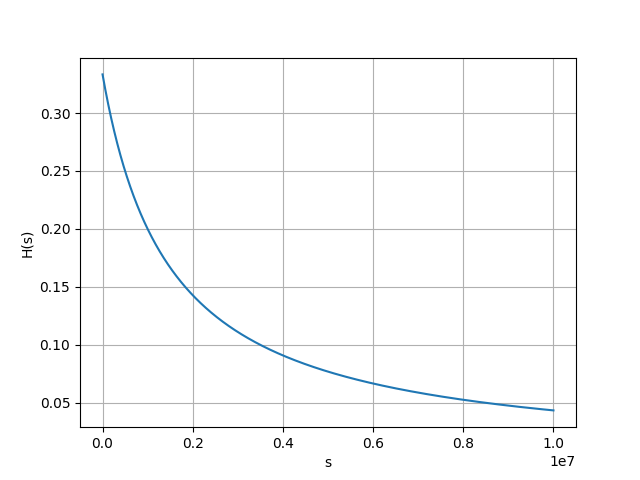
\includegraphics[width=\columnwidth]{figs/4_3.png}
    \caption{Plot of $H(s)$.}
    \label{fig:Hs}
\end{figure}
Clearly, $H(s)$ is a low-pass filter.
\item Using trapezoidal rule for integration, formulate the difference
equation by considering 
\begin{align}
	y(n) = y(t)\vert_{t=n}
\end{align}

\solution Integrating \eqref{eq:diff-eqn} between limits $n$ to $n+1$ 
and applying the trapezoidal formula,
\begin{align}
    v(n+1) - v(n) + \frac{v(n) + v(n+1)}{2\tau} = \nonumber\\
    \frac{V_2\brak{u(n)+u(n+1)}}{C_0R_2} \\
    v(n)\brak{2\tau+1} + v(n-1)\brak{2\tau-1} = \nonumber\\ 
    \frac{V_2\tau\brak{u(n)+u(n-1)}}{C_0R_2}
    \label{eq:difference-eqn}
\end{align}
for $n > 0$, where $v(0) = 0$.
\item Find $H(z)$.

\solution Note that for the input voltage, $v_i(n) = 2u(n)$ and
so, $V_i(z) = \frac{2}{1-z^{-1}}$. Applying the Z-transform
on both sides of \eqref{eq:difference-eqn},
\begin{align}
    V(z)\sbrak{(2\tau + 1) - z^{-1}(2\tau - 1)} \nonumber \\
    = \frac{\tau\brak{1 + z^{-1}}V_i(z)}{C_0R_2}
\end{align}
Hence,
\begin{align}
    H(z) = \frac{\tau\brak{1+z^{-1}}}{C_0R_2\brak{\brak{2\tau+1}-\brak{2\tau-1}z^{-1}}}
    \label{eq:Hz}
\end{align}
since $\abs{\frac{2\tau-1}{2\tau+1}} < 1$, the ROC is $\abs{z} > 1$.
\item How can you obtain $H(z)$ from $H(s)$?

\solution We use the bilinear transformation. Setting
\begin{align}
    s := \frac{2}{T}\frac{1 - z^{-1}}{1 + z^{-1}}
\end{align}
we get
\begin{align}
    H(z) &= \frac{\frac{1}{R_2}}{\frac{1}{R_1} + \frac{1}{R_2} + \frac{2C_0}{T}\frac{1 - z^{-1}}{1 + z^{-1}}} \\
         &= \frac{T\tau\brak{1+z^{-1}}}{C_0R_2\brak{\brak{2\tau+T}-\brak{2\tau-T}z^{-1}}}
\end{align}
Setting $T = 1$ gives \eqref{eq:Hz}.

\item Find $v(n)$. Verify using ngspice and the differential equation.

\solution We have,
\begin{align}
    V(z) &= H(z)V_i(z) \\
         &= \frac{TV_2\tau\brak{1+z^{-1}}}{C_0R_2\brak{1-z^{-1}}\brak{\brak{2\tau+T}-\brak{2\tau-T}z^{-1}}} \\
         &= \frac{V_2\tau\brak{z+1}}{2C_0R_2}\sum_{k=-\infty}^{\infty}\brak{1-p^k}u(k)z^{-k}
\end{align}
where $p := \frac{2\tau-T}{2\tau+T}$. Thus,
\begin{align}
    v(n) = \frac{V_2\tau}{C_0R_2}\sbrak{u(n)\brak{1-p^n}+u(n+1)\brak{1-p^{n+1}}}
\end{align}
where $p := \frac{2\tau-1}{2\tau+1}$. We take $T = 10^{-7}$ as the
sampling interval. The python code \texttt{codes/4\_7.py} verifies
these equalities.
\begin{figure}
    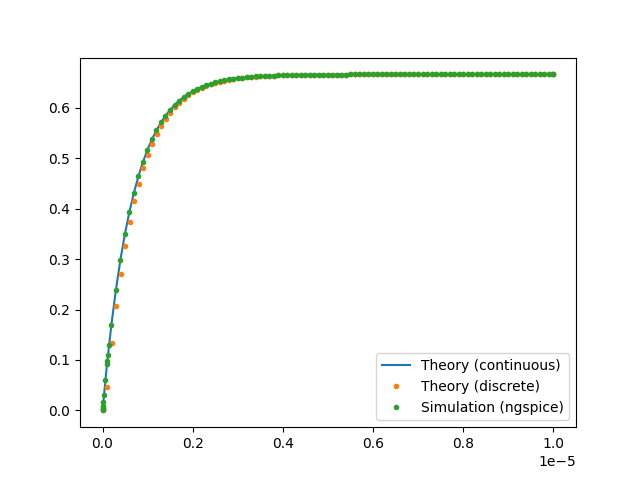
\includegraphics[width=\columnwidth]{figs/4_7.png}
    \caption{Representation of output across $C_0$.}
    \label{fig:vc0}
\end{figure}
\end{enumerate}
\end{document}
